\appendix
\clearpage

\section{Attention-Diagonal Editing Details}
\label{app:method}

\paragraph{Attention-diagonal editing.}
This appendix derives the diagonal implementation behind
Eq.~\ref{eq:unified-component-scaling}. For a general attention-row update,
\[ 
  \mathbf{y}_t=\sum_{s\le t} A_{ts}\mathbf{m}_s,\qquad
  \mathbf{y}_{t,\parallel}
  =
  \frac{\mathbf{y}_t^\top\mathbf{r}_t}{\|\mathbf{r}_t\|^2}\mathbf{r}_t .
\]
Keeping off-diagonal weights fixed, a diagonal edit gives
\(\widetilde{\mathbf{y}}_t=\mathbf{y}_t+\Delta A_{tt}\mathbf{m}_t\). Scaling
the projection of \(\mathbf{y}_t\) along \(\mathbf{r}_t\) by \(s\) therefore
requires
\[
  \Delta A_{tt}
  =
  (s-1)
  \frac{\mathbf{y}_t^\top\mathbf{r}_t}
       {\mathbf{m}_t^\top\mathbf{r}_t}.
\]
Table~\ref{tab:effective-diagonal-derivation} applies this expression to the
value-space edit and contrasts it with the residual-space attention edit.

\begin{table}[h]
  \caption{\textbf{Overview of attention-diagonal component-scaling forms.}
  The value-space edit solves a component-scaling constraint in value space.
  The residual-space attention edit instead uses the residual-space parallel
  coefficient as a diagonal correction.}
  \label{tab:effective-diagonal-derivation}
  \centering
  \footnotesize
  \setlength{\tabcolsep}{4pt}
  \begingroup
  \renewcommand{\arraystretch}{1.28}
  \resizebox{\textwidth}{!}{%
  \begin{tabular}{p{0.19\textwidth}p{0.36\textwidth}p{0.36\textwidth}}
    \toprule
    Item & Value-space objective & Residual-space objective \\
    \midrule
    Message aggregation &
    \(\displaystyle
      \mathbf{o}_t=\sum_{s\le t}A_{ts}\mathbf{v}_s
    \) &
    \(\displaystyle
      \Delta_t^{\Attn}=\sum_{s\le t}A_{ts}W_O\mathbf{v}_s
    \) \\
    Message \(\mathbf{m}_s\) &
    \(\displaystyle \mathbf{v}_s\) &
    \(\displaystyle W_O\mathbf{v}_s\) \\
    Reference \(\mathbf{r}_t\) &
    \(\displaystyle \mathbf{v}_t\) &
    \(\displaystyle \hz{}{t}\) \\
    Diagonal change &
    \(\displaystyle
      \Delta A_{tt}
      =
      (s_{\parallel}-1)
      \frac{\mathbf{o}_t^\top\mathbf{v}_t}
           {\|\mathbf{v}_t\|^2}
    \) &
    \(\displaystyle
      \Delta A_{tt}
      =
      (s_{\mathrm{res}}-1)
      \frac{(\Delta_t^{\Attn})^\top\hz{}{t}}
           {\|\hz{}{t}\|^2}
    \) \\
    Removed case &
    \(\displaystyle
      \widetilde A_{tt}
      =
      -
      \sum_{s<t}A_{ts}
      \frac{\mathbf{v}_s^\top\mathbf{v}_t}{\|\mathbf{v}_t\|^2}
    \) &
    \(\displaystyle
      \widetilde A_{tt}
      =
      A_{tt}
      -
      \sum_{s\le t}A_{ts}
      \frac{(W_O\mathbf{v}_s)^\top\hz{}{t}}
           {\|\hz{}{t}\|^2}
    \) \\
    \bottomrule
  \end{tabular}}
  \endgroup
\end{table}

\paragraph{Residual-space diagonal coefficients.}
The residual-space coefficient can be small because it is set by the
parallel part of the attention update along the residual input direction, not
by the full attention update norm. For removal,
\[
  \Delta A^{\mathrm{res}}_{tt}
  =
  -
  \frac{(\Delta_t^{\Attn})^\top\hz{}{t}}
       {\|\hz{}{t}\|^2} .
\]
The numerator is the unnormalized residual-space parallel coefficient of
\(\Delta_t^{\Attn}\), so the diagonal correction is small whenever this
parallel update is small relative to \(\hz{}{t}\).

Small magnitude does not make the edit equivalent to value-space manipulation. The
value-space objective acts on the component along \(\mathbf{v}_t\), whereas the
residual-space objective, when pulled back through \(W_O\), acts on the
component along \(W_O^\top\hz{}{t}\):
\[
  (\Delta_t^{\Attn})^\top\hz{}{t}
  =
  \mathbf{o}_t^\top W_O^\top\hz{}{t}.
\]
In general \(W_O^\top\hz{}{t}\) is not parallel to \(\mathbf{v}_t\). Therefore,
the residual-space attention edit solves a different scalar constraint from
value-space self-value-parallel manipulation. Across a sequence, each token
has its own \(\mathbf{v}_t\), \(\hz{}{t}\), and pulled-back reference
\(W_O^\top\hz{}{t}\), so the residual coefficients do not implement one
uniform scale on the value-parallel component. Compared with pure
value-space parallel scaling, the residual-space edit therefore introduces
additional motion in directions perpendicular to the self-value direction. The
zero-shot experiments indicate that this extra directional perturbation can be
harmful even when the diagonal coefficients themselves are small.

\clearpage
\section{Generated Examples Under Matched Edits}
\label{app:generation-examples}

Table~\ref{tab:generation-examples} gives qualitative generations from matched
decoding runs. All rows use the same prompt, model, decoding parameters, and
edited layer range. The value-space parallel-scaling rows stay close to the
baseline continuation. In contrast, changing the perpendicular component
produces visibly different continuations, and applying the edit in residual
space can disrupt generation even when the edit is nominally parallel.

\begin{table}[h]
  \caption{\textbf{Qualitative generation examples under residual- and
  value-space edits.}
  Each row corresponds to one setting and one generated continuation. The
  prompt and decoding configuration are fixed across rows. We show short
  surface excerpts and omit generated thinking markers when present. For the
  perpendicular rows, $s_{\parallel}$ is fixed to 1.0.}
  \label{tab:generation-examples}
  \centering
  \footnotesize
  \setlength{\tabcolsep}{4pt}
  \renewcommand{\arraystretch}{1.0}
  \begin{tabular}{p{0.15\linewidth}p{0.15\linewidth}p{0.64\linewidth}}
    \toprule
    \multicolumn{2}{p{0.30\linewidth}}{\textbf{Prompt excerpt}} &
    Malaby's tenor, Stacken's freebop piano, and Tom Rainey's drums give the
    performance a mischievous character. \\
    \midrule
    \textbf{Method} & \textbf{Scale} & \textbf{Generated continuation} \\
    \midrule
    Baseline &
    \begin{tabular}[t]{@{}l@{}}
      \(s_{\parallel}=1.0\)\\
      \(s_{\perp}=1.0\)
    \end{tabular} &
    Okay, the user provided a review of a jazz performance featuring
    Malaby's tenor saxophone and pianist Stacken, along with drummer Tom Rainey. \\
    \addlinespace[0.25em]
    \midrule
    \multirow{3}{*}{Value-space} & $s_{\parallel}=-1.0$ &
    Okay, the user provided a review of a jazz performance featuring
    Malaby's tenor saxophone and pianist Stacken, along with drummer Tom Rainey. \\
    & $s_{\parallel}=0.0$ &
    Okay, the user provided a review of a jazz performance featuring
    Malaby's tenor saxophone and pianist Stacken, along with drummer Tom Rainey. \\
    & $s_{\parallel}=2.0$ &
    Okay, the user provided a review of a jazz performance featuring
    Malaby's tenor sax and Stacken's piano, with drummer Tom Rainey. \\
    \addlinespace[0.25em]
    \midrule
    \multirow{3}{*}{Residual-space} & $s_{\perp}=0.0$ &
    National, nowbce bridge, CellValue, SherSources, Bes Chambers,
    JPioldc, malformed tokens, fragmented phrases, craft look \ldots \\
    & $s_{\perp}=0.5$ &
    Jean Caesar once said: history is not about whether it is important,
    but whether it is told. Is this line from The Fall of Ulyssias? \\
    & $s_{\perp}=1.5$ &
    Okay, let me try to unpack this review. The user is asking for an analysis
    of a jazz performance by Malaby and Stacken. \\
    \bottomrule
  \end{tabular}
\end{table}

\clearpage
\section{Additional Editing Results}
\label{app:additional-editing}

\paragraph{Zero-shot parallel editing.}
Table~\ref{tab:appendix-ruler-full} expands the RULER long-context evaluation
by task family and sequence length for Llama-3.2-3B. This view complements the
main-text average table: V-Para Rem. remains close to baseline within each
family, whereas residual-space parallel removal degrades several subdomains,
especially at longer context lengths.

\begin{table}[h]
  \caption{\textbf{Full long-context RULER benchmark breakdown by task family
  and context length.}
  Scores are reported for Llama-3.2-3B across the 4k--128k context-length
  sweep. Attn/MLP/Both Para-Rem. denote residual-space parallel removal on
  the corresponding branch(es); V-Para Rem. denotes value-space parallel
  removal.}
  \label{tab:appendix-ruler-full}
  \centering
  \scriptsize
  \setlength{\tabcolsep}{2.4pt}
  \begin{minipage}{0.49\linewidth}
    \centering
    \resizebox{\linewidth}{!}{%
    \begin{tabular}{lrrrrrr}
      \toprule
      Setting & 4k & 8k & 16k & 32k & 64k & 128k \\
      \midrule
      \multicolumn{7}{l}{\textbf{NIAH}} \\
      Baseline & 99.3 & 97.6 & 93.9 & 90.3 & 85.7 & 83.9 \\
      Attn Para-Rem. & 96.5 & 95.3 & 90.4 & 85.8 & 81.2 & 77.5 \\
      MLP Para-Rem. & 72.4 & 61.1 & 56.8 & 52.0 & 49.6 & 43.5 \\
      Both Para-Rem. & 84.8 & 71.5 & 62.6 & 55.5 & 53.0 & 48.0 \\
      V-Para Rem. & 99.4 & 97.7 & 94.0 & 90.7 & 85.9 & 83.9 \\
      \midrule
      \multicolumn{7}{l}{\textbf{QA}} \\
      Baseline & 55.0 & 49.6 & 49.0 & 48.1 & 41.8 & 39.9 \\
      Attn Para-Rem. & 45.7 & 40.5 & 42.3 & 42.8 & 36.9 & 35.8 \\
      MLP Para-Rem. & 40.4 & 32.0 & 28.0 & 26.5 & 20.4 & 16.3 \\
      Both Para-Rem. & 44.1 & 36.7 & 31.3 & 31.6 & 24.7 & 20.3 \\
      V-Para Rem. & 54.6 & 49.4 & 49.3 & 48.5 & 42.2 & 39.6 \\
      \midrule
      \multicolumn{7}{l}{\textbf{VT}} \\
      Baseline & 96.8 & 93.6 & 91.6 & 91.2 & 87.3 & 82.9 \\
      Attn Para-Rem. & 71.0 & 70.2 & 69.3 & 69.6 & 71.2 & 63.5 \\
      MLP Para-Rem. & 39.6 & 44.0 & 44.8 & 22.2 & 16.2 & 6.1 \\
      Both Para-Rem. & 57.7 & 57.8 & 61.4 & 40.3 & 28.8 & 9.8 \\
      V-Para Rem. & 96.1 & 93.0 & 91.4 & 91.0 & 87.8 & 83.2 \\
      \bottomrule
    \end{tabular}}
  \end{minipage}\hfill
  \begin{minipage}{0.49\linewidth}
    \centering
    \resizebox{\linewidth}{!}{%
    \begin{tabular}{lrrrrrr}
      \toprule
      Setting & 4k & 8k & 16k & 32k & 64k & 128k \\
      \midrule
      \multicolumn{7}{l}{\textbf{CWE}} \\
      Baseline & 48.0 & 11.3 & 5.8 & 1.1 & 0.6 & 0.9 \\
      Attn Para-Rem. & 18.6 & 8.3 & 5.3 & 2.0 & 0.5 & 0.3 \\
      MLP Para-Rem. & 20.6 & 8.6 & 4.8 & 2.9 & 1.9 & 2.5 \\
      Both Para-Rem. & 49.1 & 30.6 & 15.0 & 6.0 & 3.5 & 2.8 \\
      V-Para Rem. & 44.0 & 9.8 & 5.4 & 1.0 & 0.6 & 0.9 \\
      \midrule
      \multicolumn{7}{l}{\textbf{FWE}} \\
      Baseline & 86.7 & 76.1 & 85.2 & 88.5 & 78.6 & 66.3 \\
      Attn Para-Rem. & 31.3 & 28.3 & 37.2 & 42.0 & 36.3 & 21.6 \\
      MLP Para-Rem. & 16.3 & 9.3 & 3.7 & 14.6 & 1.3 & 2.4 \\
      Both Para-Rem. & 48.6 & 41.3 & 37.9 & 38.5 & 14.5 & 22.7 \\
      V-Para Rem. & 86.7 & 76.7 & 86.0 & 87.9 & 79.6 & 66.9 \\
      \midrule
      \multicolumn{7}{l}{\textbf{Overall}} \\
      Baseline & 77.2 & 65.6 & 65.1 & 63.8 & 58.8 & 54.8 \\
      Attn Para-Rem. & 52.6 & 48.5 & 48.9 & 48.4 & 45.2 & 39.7 \\
      MLP Para-Rem. & 37.9 & 31.0 & 27.6 & 23.6 & 17.9 & 14.2 \\
      Both Para-Rem. & 56.9 & 47.6 & 41.6 & 34.4 & 24.9 & 20.7 \\
      V-Para Rem. & 76.2 & 65.3 & 65.2 & 63.8 & 59.2 & 54.9 \\
      \bottomrule
    \end{tabular}}
  \end{minipage}
\end{table}

Table~\ref{tab:appendix-zeroshot-parameter-sweeps} gives a per-task view of
fixed value-parallel scaling on Qwen3-4B. Together with the RULER breakdown,
it serves as additional zero-shot evidence for the editing experiments:
moderate value-parallel scaling is mostly stable across tasks, but it does not
produce a reliable task-level improvement.

\begin{table}[h]
  \caption{\textbf{Ablation study on value-parallel scale ratios for Qwen3-4B
  zero-shot evaluation.}
  Scores are grouped by non-generative and generative task families.}
  \label{tab:appendix-zeroshot-parameter-sweeps}
  \centering
  \scriptsize
  \setlength{\tabcolsep}{3pt}
  \resizebox{\textwidth}{!}{%
  \begin{tabular}{lrrrrrrrrrrrrrr}
    \toprule
    \multirow{2}{*}{$s_{\parallel}$}
    & \multicolumn{7}{c}{Non-generative}
    & \multicolumn{6}{c}{Generative}
    & \multirow{2}{*}{\underline{Avg.}} \\
    \cmidrule(lr){2-8}\cmidrule(lr){9-14}
    & OBQA & PIQA & WinoGr & BoolQ & ARC-C & HSwag & MMLU & GSM8K & HumanEval & NQ & DROP & MBPP & BBH & \\
    \midrule
    $-3.0$ & 40.6 & 75.2 & 67.2 & 85.0 & 62.1 & 69.5 & 58.0 & 84.4 & 71.3 & 15.4 & 10.1 & 64.0 & 79.6 & 60.2 \\
    $-1.0$ & 40.4 & 75.0 & 66.8 & 85.1 & 61.8 & 69.7 & 62.0 & 84.6 & 73.2 & 15.6 & 10.0 & 63.4 & 82.0 & 60.7 \\
    $0.0$ & 39.8 & 74.6 & 67.8 & 85.1 & 62.0 & 69.8 & 60.0 & 85.4 & 73.8 & 15.9 & 9.9 & 62.4 & 77.6 & 60.3 \\
    $0.5$ & 40.0 & 75.1 & 67.6 & 85.2 & 62.2 & 69.7 & 61.0 & 84.9 & 72.0 & 15.8 & 9.8 & 62.8 & 79.2 & 60.4 \\
    $1.0$ & 33.4 & 72.5 & 64.4 & 62.2 & 47.1 & 69.6 & 59.0 & 84.5 & 73.2 & 15.9 & 10.0 & 62.2 & 84.0 & 56.8 \\
    $1.5$ & 40.4 & 74.7 & 67.4 & 85.0 & 61.6 & 69.6 & 61.0 & 85.0 & 72.0 & 15.7 & 9.9 & 62.0 & 82.8 & 60.5 \\
    $2.0$ & 40.2 & 75.1 & 67.2 & 85.0 & 61.6 & 69.7 & 60.0 & 85.1 & 72.0 & 15.7 & 9.9 & 62.4 & 80.4 & 60.3 \\
    $3.0$ & 41.0 & 74.9 & 67.2 & 85.1 & 61.9 & 69.7 & 62.0 & 84.7 & 69.5 & 15.6 & 10.0 & 63.8 & 79.6 & 60.4 \\
    $5.0$ & 40.8 & 75.2 & 67.6 & 85.2 & 62.1 & 69.6 & 63.0 & 85.2 & 70.1 & 15.4 & 9.7 & 63.6 & 81.2 & 60.7 \\
    \bottomrule
  \end{tabular}}
\end{table}

\clearpage
\section{Pretraining Configuration Details}
\label{app:training-configs}

Table~\ref{tab:appendix-training-configs} summarizes the model and training
configurations for the scratch pretraining runs used in
Section~\ref{sec:pretraining}. The small GPT-style sweep uses OpenWebText
training data and runs for 600k updates, corresponding to roughly 300B
tokens. The larger runs use FineWeb100BT and follow a 100B-token schedule.

\begin{table}[h]
  \caption{\textbf{Pretraining model and optimization configurations.}
  We list the training data and model sizes used in the scratch pretraining
  runs.}
  \label{tab:appendix-training-configs}
  \centering
  \small
  \setlength{\tabcolsep}{6pt}
  \begin{tabular}{llrrr}
    \toprule
    Training data & Params & Layers & Heads & Width \\
    \midrule
    \multirow{5}{*}{OpenWebText}
      & 194M & 12 & 14 & 896  \\
      & 241M & 14 & 15 & 960  \\
      & 296M & 14 & 16 & 1024 \\
      & 436M & 16 & 18 & 1152 \\
      & 528M & 18 & 20 & 1280 \\
    \midrule
    \multirow{2}{*}{FineWeb100BT}
      & 1.4B & 24 & 16 & 2048 \\
      & 2.7B & 32 & 20 & 2560 \\
    \bottomrule
\end{tabular}
\end{table}

These configurations cover the small-model loss curves in
Figure~\ref{fig:pretraining} and the larger downstream summaries in
Table~\ref{tab:pretraining-summary}. The reduced table focuses on architecture
because the dataset and token budgets are shared within each group.

\paragraph{Training-side gated scaling diagnostic.}
Figure~\ref{fig:appendix-1p4-trainable-scale} compares 1.4B training traces
for baseline training, fixed V-Para Rem., and a gated parallel-scaling
variant. The gated variant predicts a tokenwise scalar gate from the hidden
state using a learned \(d\!\to\!1\) projection and uses it to modulate the
parallel component. This auxiliary run does not show a stable advantage over
the fixed removal baseline. We therefore treat gated parallel scaling as a
diagnostic variant rather than a method contribution.

\begin{figure}[h]
  \centering
  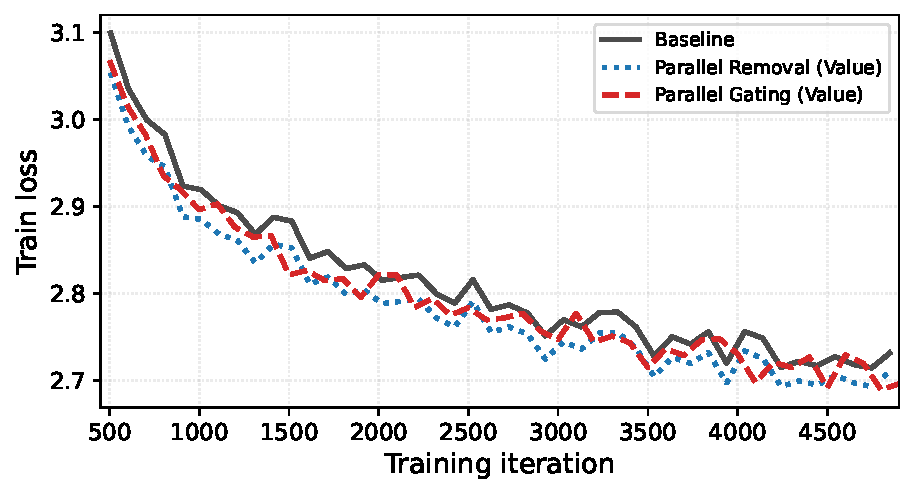
\includegraphics[width=0.68\linewidth]{figs/loss_curves/loss_1p4_gate_vs_xsa_absolute.pdf}
  \caption{\textbf{Ablation study on parallel-scale adjustment during 1.4B
  pretraining.}
  Curves compare baseline training, fixed V-Para Rem., and a gated
  parallel-scale adjustment.}
  \label{fig:appendix-1p4-trainable-scale}
\end{figure}

\clearpage
\section{Extended Compression Geometry}
\label{app:compression}

Figures~\ref{fig:appendix-compression-perp} and
\ref{fig:appendix-compression-para} supplement the main-text compression
result with additional views of the same local-flip analysis. The first figure
reports the layer-wise update magnitude from the uncompressed model and the
perpendicular error in the block and MLP branches. The second figure reports
the corresponding parallel-error share across branches. Together, these views
show that quantization produces visibly smaller deviations, while stronger
pruning separates more clearly in the direction-changing component. The
parallel component is less discriminative on its own, but it completes the
integrated view of how compression error decomposes across branches.

\begin{figure}[h]
  \centering
  \begin{minipage}{0.32\textwidth}
    \centering
    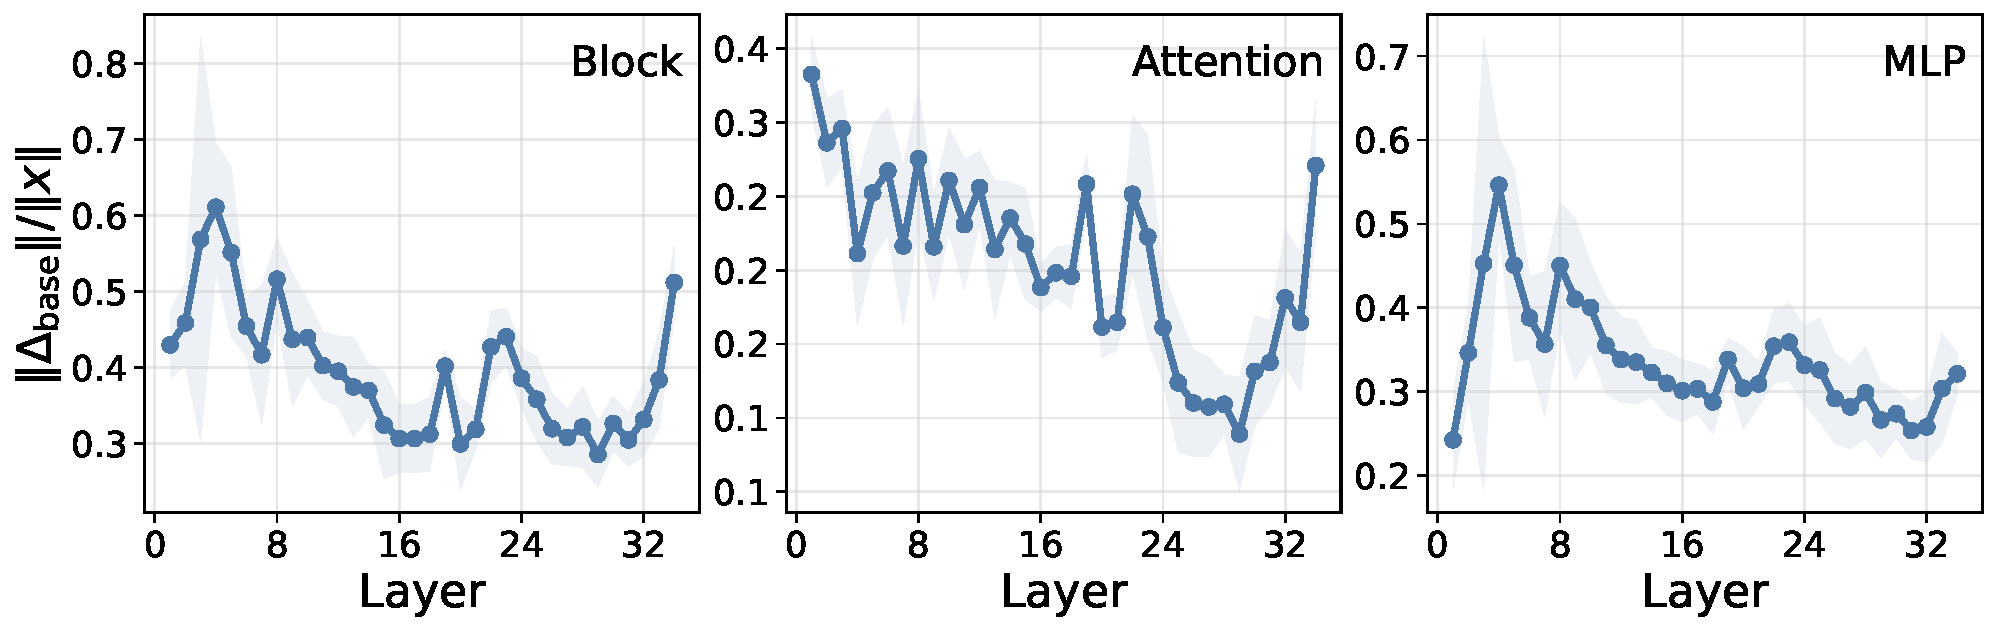
\includegraphics[width=\linewidth]{figs/comp_analysis/baseline_update_over_hidden_state.pdf}
  \end{minipage}\hfill
  \begin{minipage}{0.32\textwidth}
    \centering
    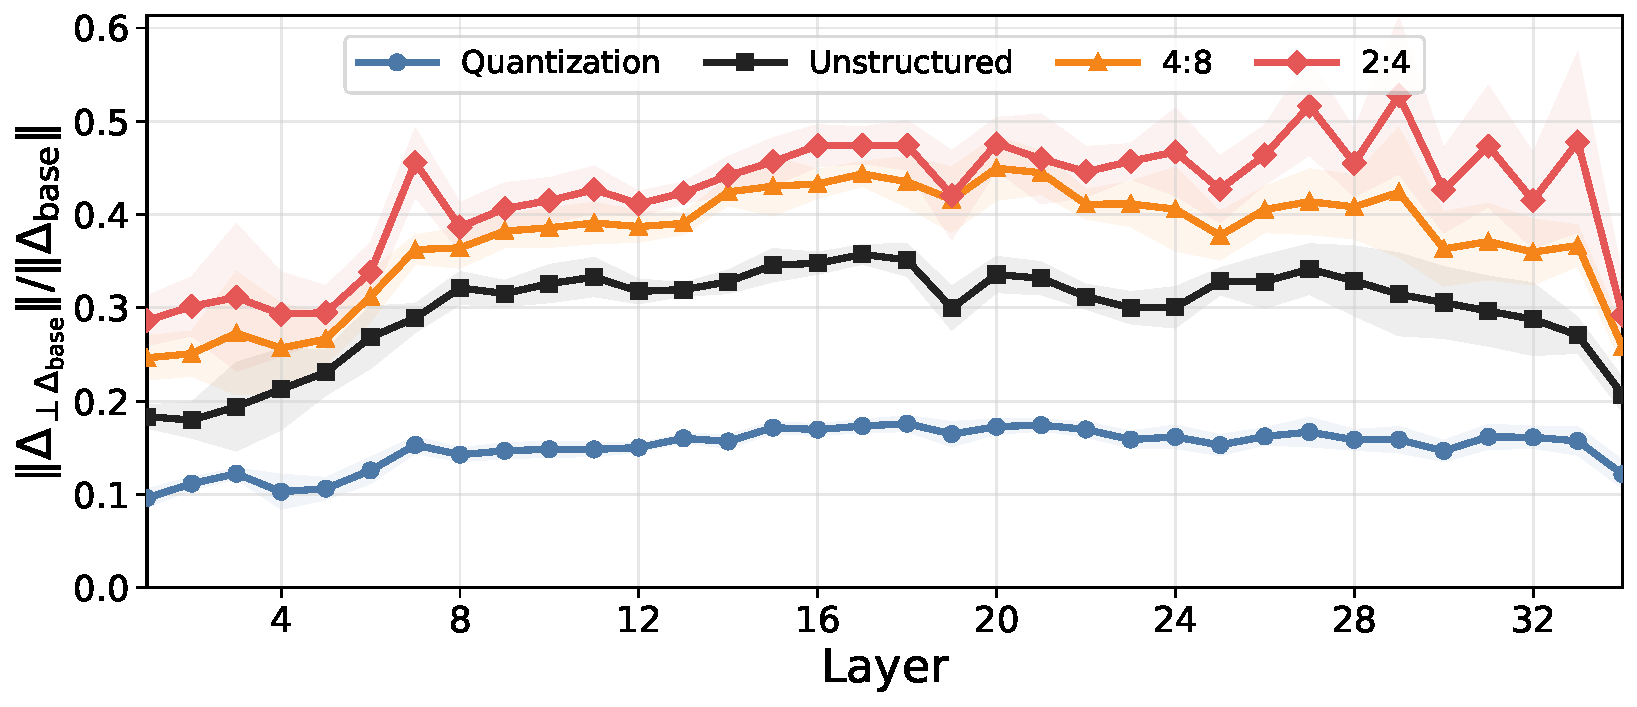
\includegraphics[width=\linewidth]{figs/comp_analysis/local_flip_compare-block_out-perp_over_base_update.pdf}
  \end{minipage}\hfill
  \begin{minipage}{0.32\textwidth}
    \centering
    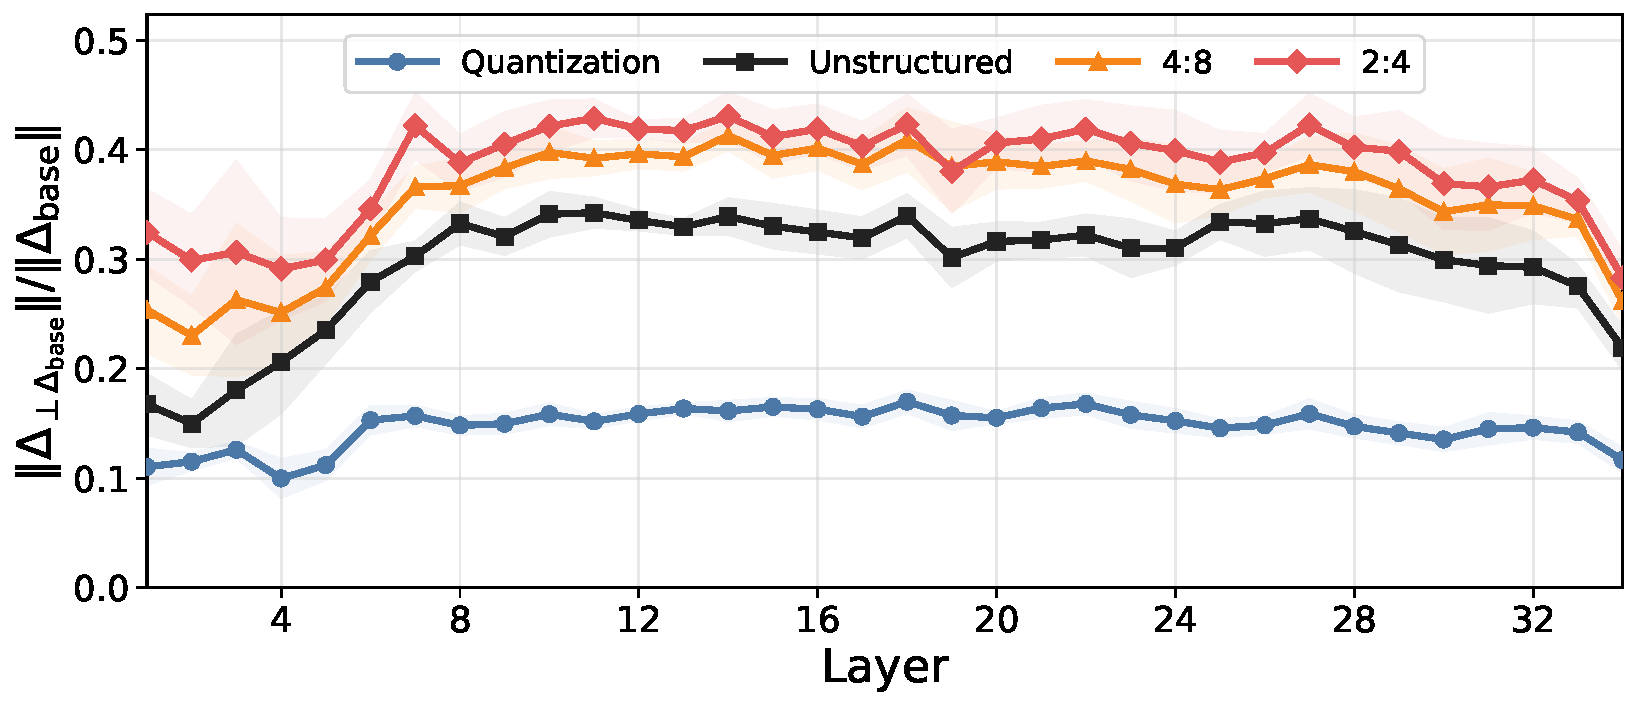
\includegraphics[width=\linewidth]{figs/comp_analysis/local_flip_compare-mlp_out-perp_over_base_update.pdf}
  \end{minipage}
  \caption{\textbf{Compression-geometry breakdown across branches.}
  Left: uncompressed-model update magnitude, normalized by hidden-state
  magnitude. Middle/right: perpendicular share of block- and MLP-output
  compression error.}
  \label{fig:appendix-compression-perp}
\end{figure}

\begin{figure}[h]
  \centering
  \begin{minipage}{0.32\textwidth}
    \centering
    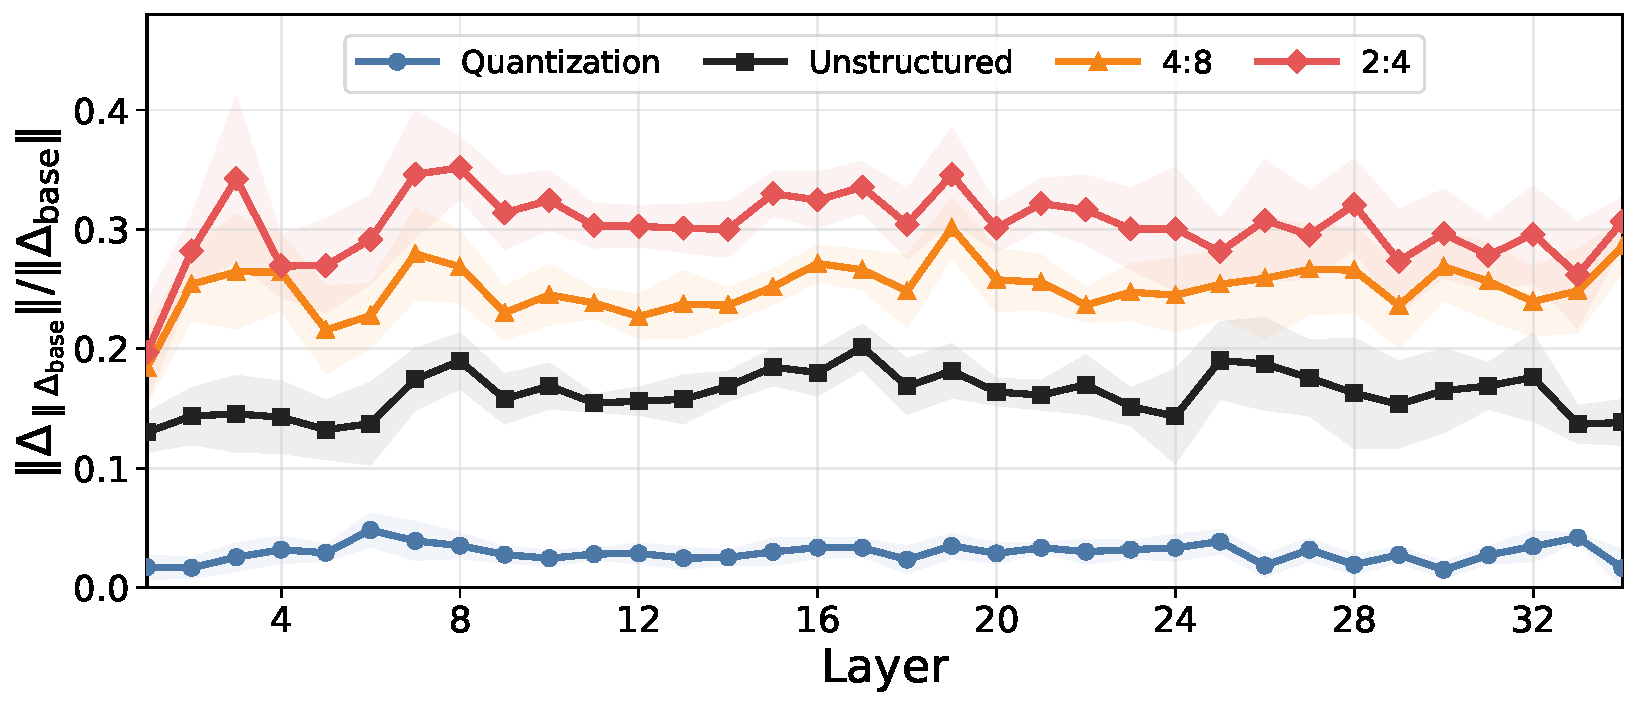
\includegraphics[width=\linewidth]{figs/comp_analysis/local_flip_compare-block_out-para_over_base_update.pdf}
  \end{minipage}\hfill
  \begin{minipage}{0.32\textwidth}
    \centering
    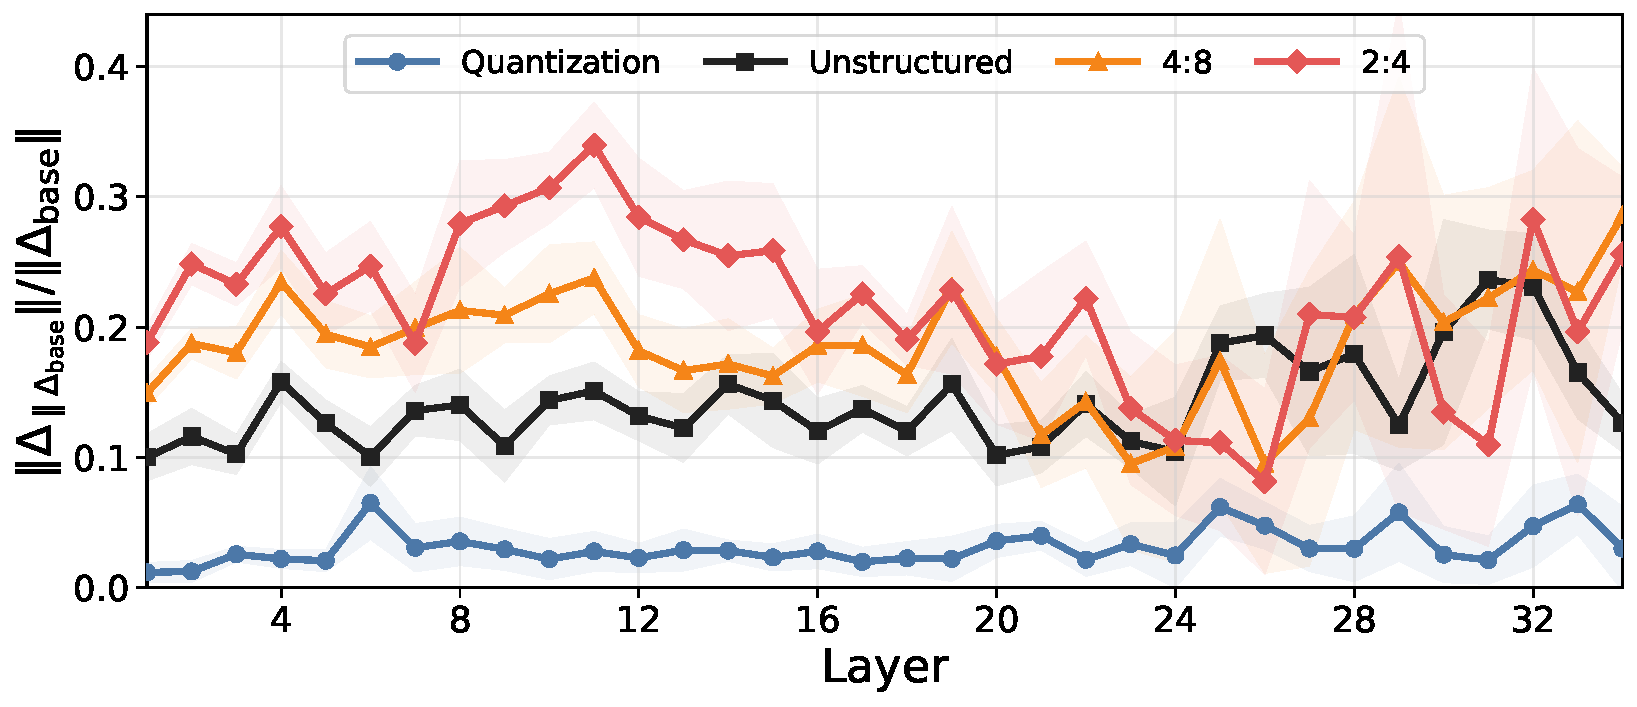
\includegraphics[width=\linewidth]{figs/comp_analysis/local_flip_compare-attn_out-para_over_base_update.pdf}
  \end{minipage}\hfill
  \begin{minipage}{0.32\textwidth}
    \centering
    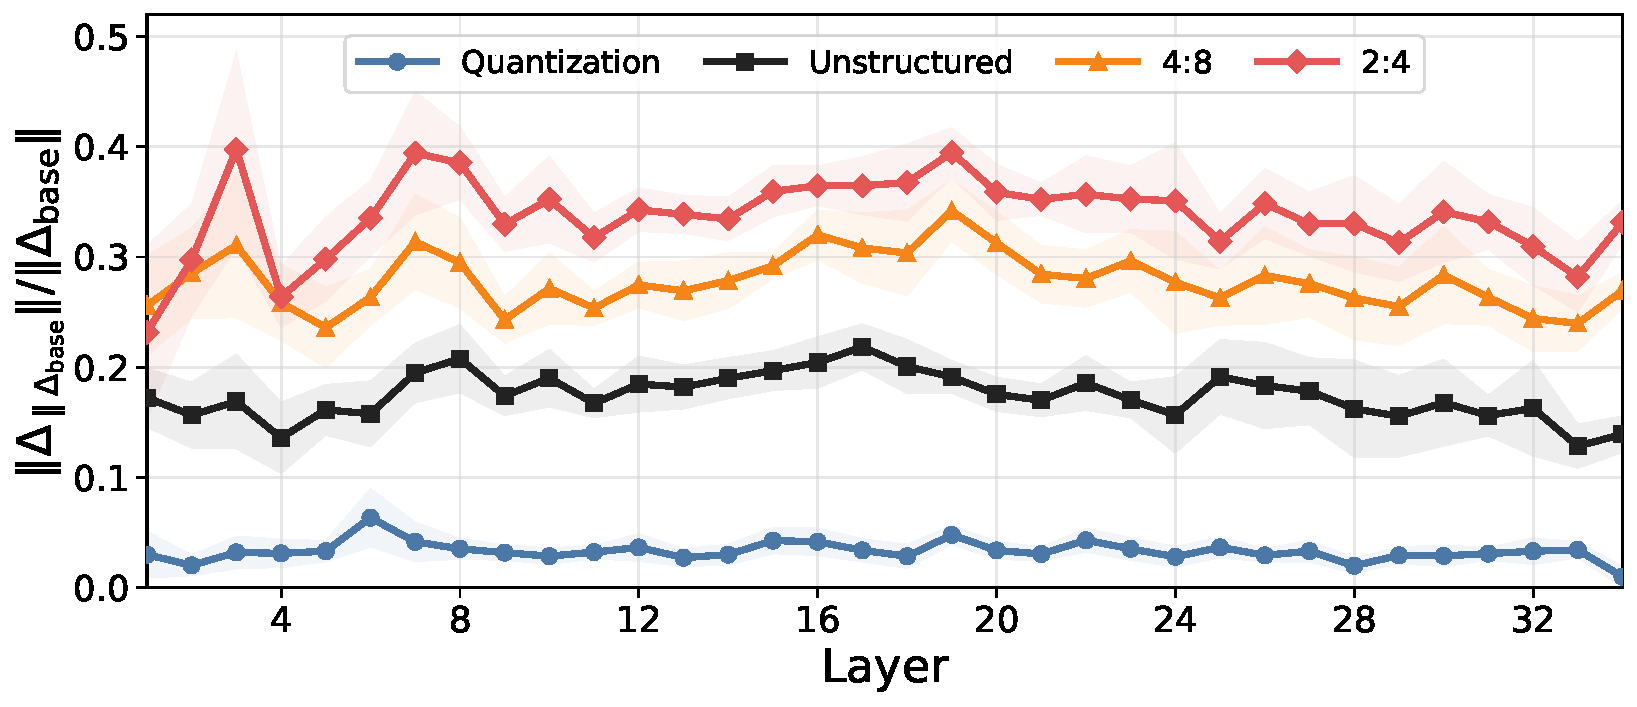
\includegraphics[width=\linewidth]{figs/comp_analysis/local_flip_compare-mlp_out-para_over_base_update.pdf}
  \end{minipage}
  \caption{\textbf{Parallel-error breakdown under compression.}
  Left/middle/right: parallel share of block-, attention-, and MLP-output
  compression error.}
  \label{fig:appendix-compression-para}
\end{figure}
